\section{Applications of parallel multilinear detection}
\label{sec:applications}

Multilinear detection has a broad class of applications, two of which we discuss here.
The first involves finding paths and trees in a graph---Koutis et al.
\cite{DBLP:journals/talg/KoutisW16} showed that these problems can be solved using
multilinear detection. We describe how Algorithm \parmaxwt{} can be adapted
to solve this problem. The second problem involves anomaly detection using the
approach known as graph scan statistics. This was solved sequentially using 
the color coding technique in \cite{cadena:sdm17}; we show how this entire class
of problems can be solved by adapting Algorithm \parmaxwt{}.
As before, $G = (V, E)$, denotes a graph where $V$ is a set of $n$ vertices or nodes, and 
$E$ is a set of $m$ edges. Let $\nbr{v}=\{u: (u,v)\in E\}$ denote the set of neighbors
of node $v$.

\subsection{Finding Paths and Trees}
\label{sec:apps-trees}

%We consider a more general, weighted version of the problem. We assume a weight $w(v)$
%for each node $v\in V$.
Given a graph $G=(V, E)$ with $n=|V|$, $m=|E|$, and a subgraph $H=(V_H, E_H)$, with $k=|V_H|$,
the basic subgraph isomorphism problem involves finding a mapping $f:V_H\rightarrow V$
such that $(i, j)\in E_H$ if and only if $(f(i), f(j))\in E$. 

\begin{problem} ($k$-Tree)
\label{prob:trees}
Given a weighted graph $G=(V, E)$ with a weight vector $\mathbf{w}$, and a tree
denoted by $H=(V^H, E^H)$ with $|V^H|=k$, the objective is to determine if there exists
an embedding of $H$ in $G$.
\end{problem}

We show below that problem \ref{prob:trees} can be solved by Algorithm \parmaxwt{} 
by formalizing this as a multilinear detection problem. We first consider the case
where $H$ is a path of length $k$, for notational simplicity.
Let $x_v$ denote a variable associated with each node $v\in V$.
We define poynomials $P_v(i)$ for all $v\in V$, $i\leq k$ in the following manner.

\begin{itemize}
\item
$P_v(1) = x_v$ for all $v\in V$
\item
For $i>1$,
$P_v(i) = \sum_{i'<i} \sum_{u\in\nbr(v)} P_u(i')P_v(i-i')$
\item
Define the polynomial $P(x_1,\ldots,x_n) = \sum_v P_v(k)$
\end{itemize}

It can be verified that the graph $G$ has a path of length $k$ if and only if the
polynomial $P(x_1,\ldots,x_n)$ has a multilinear term.


\begin{figure}[h]
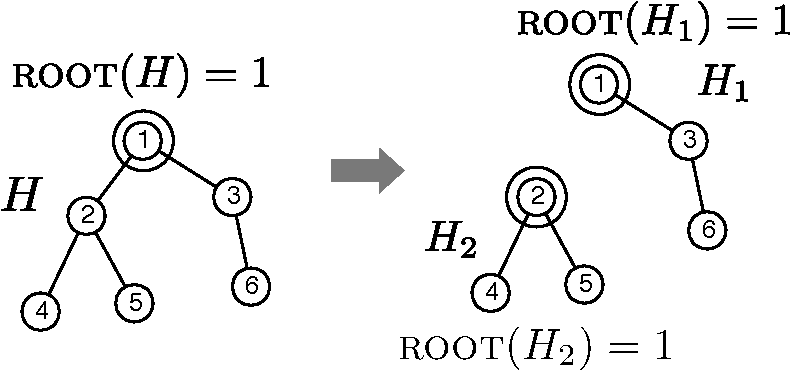
\includegraphics[width=0.4\textwidth]{img/trees.pdf}
\caption{
\small
Tree $H$ with $\myroot(H)=1$. It is decomposed into trees $H_1$ and $H_2$ by
removing the edge $(1, 2)$. $\myroot(H_1)=1$ and $\myroot(H_2)=2$.
%\vspace{-0.2in}
}
\label{fig:trees}
\end{figure}
Next, we consider the case where $H$ is a tree. We consider the tree to be rooted,
and let $\myroot(H)$ be the root node, selected arbitrarily. We consider a hierarchical
structure among subtrees of $H$ in the following manner: consider any node $u\in\nbr(\myroot(H))$.
Let $H_1$ and $H_2$ denote the subtrees obtained upon deleting the edge $(u, \myroot(H))$,
with $\myroot(H)\in H_1$ and $u\in H_2$. We set $\myroot(H_1)=\myroot(H)$ and $\myroot(H_2)=u$.
This process is illustrated i Figure \ref{fig:trees}.
The subtrees $H_1$ and $H_2$ are further partitioned in a recursive manner, till
all trees have a single node. For an intermediate tree $H'$ in this process,
let $\textsc{child}_1(H')$ and $\textsc{child}_2(H')$ denote the two child trees
resulting from the tree $H'$. Let $\textsc{parent}(H')=H''$ be the tree such that
either $\textsc{child}_1(H'')= H'$ or $\textsc{child}_2(H'') = H'$.
We define the polynomials $P_v(H')$, which will correspond to all layouts (not necessarily
isomorphisms) of $H'$ with $\myroot(H')=v$, in the following manner:
\begin{itemize}
\item
If $H'$ consists of a single node, $P_v(H') = x_v$
\item
Else, 
$P_v(H') = \sum_{u\in\nbr(v)} P_v(H'_1)P_u(H'_2)$, where
$H'_1$ and $H'_2$ denote $\textsc{child}_1(H')$ and $\textsc{child}_2(H')$, respectively.
\item
Finally, we have
$P(x_1,\ldots, x_n)= \sum_v P_v(H)$
\end{itemize}

More generally, we consider a weighted version of the problem, where the goal is to
find an embedding of the maximum weight. 

\subsection{Anomaly Detection Using Graph Scan Statistics}
\label{sec:apps-scanstat}

We use the notation of \cite{cadena:sdm17} here. We assume each node $v\in V$ has two associated values,
which vary with time (we will not show the time, to avoid complicating the notation):
(1) a \emph{baseline count}, $b(v)$, which indicates the count that we 
expect to see at the node $v$---e.g., the number of people in a county corresponding to node $v$---and
(2) an \emph{event count} or \emph{weight}, $w(v)$, which indicates how many occurrences of an event 
of interest are seen at the node---e.g., the number of cases of a disease in a county.

Graph scan statistics are among the most commonly used methods for detecting anomalies or ``hotspots" in 
networked data \cite{Speakman-14,leiserson2015pan, hansen2016finding, neil2013scan, chen2014non}. 
Informally, this approach formalizes anomaly detection as a hypothesis testing problem.
Under the null hypothesis $H_0$, it is \emph{business as usual}, and the event counts for all nodes are generated proportionally to their baseline counts. Under the alternative hypothesis $H_1(S)$, counts of a majority of
the vertices are generated (again) with rate proportional to the baseline counts, but there exists a small connected subset
$S \subseteq V$ of vertices for which the counts are generated at a higher rate than expected.
Then, the goal is to find a set of vertices $S$ that maximizes an appropriate scan statistic function $F(S)$, typically a log-likelihood ratio that compares event counts to baseline counts. We define a scan statistic in terms of the event and baseline counts of a node set:
$$
F(S) = F(W(S), B(S), \mathbf{\theta}),
$$
where $W(S) = \sum_{v \in S} w(v)$ is the total event count or \emph{weight} of $S$, $B(S) = \sum_{v \in S} b(v)$ is the baseline count of the set, and $\theta$ represents possible additional arguments to $F$.

Depending on the assumptions that are satisfied by the data, there are two broad types of scan statistics: parametric and non-parametric. 
An example of a non-parametric function is the Berk-Jones scan statistic (BJ) \cite{Berk-79} used for civil unrest events and network intrusion detection~\cite{chen2014non,mcfowland2013fast}. In this setting, each node $v$ has a $p$-value $p(v) \in [0,1]$, and, for a significance level $\alpha$, the event count $w(v)$ is 1 if $p(v) < \alpha$ (i.e., the node is significant) and 0 otherwise, and the baseline count is $b(v) = 1$ for all nodes. This scan statistic is defined as
{\scriptsize
$$
\max_{\alpha \leq \alpha_{max}}B(S) \left[\frac{W(S)}{B(S)} \log\left(\frac{\frac{W(S)}{B(S)}}{\alpha}\right) + \left(1 - \frac{W(S)}{B(S)}\right) \log\left(\frac{1 - \frac{W(S)}{B(S)}}{1 -\alpha}\right) \right],
$$}
with $\mathbf{\theta} = \alpha_{max}$.
A well-known example of a parametric function is the Kulldorff scan statistic commonly used in disease surveillance \cite{kulldorff_spatial_1997,Duczmal06,kulldorff2003power,neill-jss12}, which is defined as 
{\scriptsize $$
W(S) \log\left(\frac{W(S)}{B(S)}\right) + (W(V) - W(S)) \log\left(\frac{W(V) - W(S)}{B(V) - B(S)}\right) - C(V) \log\left(\frac{W(V)}{B(V)}\right),
$$}
with $\mathbf{\theta} = (W(V),B(V))$. 
A number of other scan statistics are discussed in \cite{cadena:sdm17}. Our methods will extend to
all of those. We also note that the suitability of scan statistics depends on the application and the assumptions
underlying the dataset. We refer to
\cite{margai2003community, neill-jss12, kulldorff_spatial_1997, neill2007nonparametric}
for a more detailed discussion of the advantages and limitations
of these approaches, since this is not the focus of our paper.

\noindent
\textbf{Problem Formulation} 
The graph anomaly detection problem can be posed as the following constrained optimization problem,
which has been shown to be NP-hard, in general \cite{cadena:sdm17}.

\begin{problem}
\label{prob:macs}
Given a graph $G=(V, E)$, a scan statistic $F(\cdot)$, the associated counts for vertices---$\mathbf{w}$ and $\mathbf{b}$---and a parameter $k$, find a connected subset $S\subseteq V$ that maximizes $F(S) = F(W(S), B(S), \theta)$ with $B(S) \leq k$.
\end{problem}

\noindent
\textbf{Reduction to multilinear detection on a DAG.}
We define the sets $K=\{1,2 \ldots, k\}$ where $k$ is a \emph{size parameter}, 
and $R=\{0,1,2,\ldots, r\}$, where $r$ is a \emph{weight parameter}. Let $w(v)$ denote the
weight for each node $v\in V$; the weights are binned by considering powers of $(1+\epsilon)$, for an error parameter $\epsilon>0$: if $w(v)\in [(1+ \epsilon)^{j-1}, (1+ \epsilon)^{j})$, we will sometimes say that $v$ is
in the weight group $j$; this definition is extended to the weight of a subgraph.

For each node $v$, we define a variable $x_v$, and we construct a polynomial over the set of variables $\{x_v: v \in V\}$. Every term---i.e., monomial---in this polynomial will represent a connected subgraph of size at most $k$ and weight at most $(1+ \epsilon)^r$. 
For $i \in K$ and $j \in R$, let $P_v(i,j)$ be the polynomial corresponding to a subgraph (1) containing node $v$, (2) of size $i$, and (3) total weight in 
$[(1+ \epsilon)^{j-1}, (1+ \epsilon)^{j})$. $P_v(i,0)$ represents subgraphs of weight 0.
The following recurrence relations describe how the polynomials $P_v(i, j)$ are computed:
\begin{itemize}
\item
$P_v(i, j) = \bar{0}$ for $i \in K$, $j \in R$
\item
$P_v(1, j) = x_v$ for all $v \in V$, $j = \lceil \log_{(1 + \epsilon)} (w(v) + 1)\rceil$
\item
for $v \in V$, $i = 2$ to $k$, $j = 0$ to $r$:
\begin{itemize}
\item
if $j=0$: $P_v(i,0) = \sum_{u \in \nbr(v)} \sum_{i' = 1}^i (P_v(i',0) \cdot P_u(i-i', 0))$ 
\item
if $j=1$:
$P_v(i,1) = \sum_{u \in \nbr(v)} \sum_{i' = 1}^i (P_v(i', 1) \cdot P_u(i-i', 0) + (P_v(i', 0) \cdot P_u(i-i', 1))$
\item
if $j\geq 2$:
$P_v(i,j) = \sum_{u \in \nbr(v)} \sum_{i' = 1}^i (P_v(i', j - 1) \cdot P_u(i-i', j - 1) +
P_v(i', j) \cdot P_u(i-i', 0) + P_v(i', 0) \cdot P_u(i-i', j))$
\end{itemize}
\item
$P(i,j) = \sum_v P_v(i,j)$ for $i \in K$, $j \in R$
\end{itemize}

The above computation can be represented as a polynomial described by a DAG, in which the
nodes corresponding to $P_v(i, j)$ are the intermediate nodes, which are computed by ``$\cdot$'' and ``$+$''
operations.
